%\section{Доказательство будем вести от приятного!}

Во \textbf{второй главе} рассмотрена задача о смене ролика в контакте с опорной плоскостью. При повороте колеса вокруг своей оси на достаточно большой угол находящийся в контакте с опорной плоскостью ролик перестает с ней контактировать. В контакт с плоскостью приходит новый ролик, скорость которого, вообще говоря, не согласована со связями. При этом возникает переходный процесс, во время которого возможно скольжение ролика относительно опорной плоскости. В данной главе предполагается, что скольжение ролика прекращается за бесконечно малый промежуток времени. Составлены линейные алгебраические уравнения, определяющие обобщенные скорости после смены ролика в контакте в соответствии с теорией удара. Таким образом, для получения движений экипажа требуется найти решения задачи Коши уравнений, полученных в первой главе, на интервалах, где в контакте находится один и тот же ролик, и решения линейных алгебраических уравнений при сменах роликов для получения начальных условий для следующих гладких участков. Получены и проанализированы численные решения для симметричной конфигурации экипажа.

%При рассмотрении динамики роликов отдельного внимания заслуживает момент перехода колеса с одного ролика на другой, поскольку вращение ролика, входящего в контакт, может не быть согласовано с условием отсутствия скольжения в контакте.

%В данной главе проведено детальное рассмотрение момента смены ролика в контакте с учетом ударного характера взаимодействия с опорной плоскостью. Также, получены численные решения, состоящие из участков, определяемых уравнениями движения, и моментов смены контакта, моделируемых с точки зрения теории удара.

\begin{figure}
    \minipage{\textwidth}
        \centering
        \asyinclude{./content/pic/asy/pic_overlap.asy}
        \caption{Омни-колесо в рассматриваемой конфигурации. Концы роликов усечены. Имеется пренебрежимое пересечение тел роликов.}
        \label{fig:overlap}
    \endminipage
\end{figure}

% Уравнения движения системы, полученные в первой главе, описывают динамику системы в тех интервалах времени, когда ролик в контакте с опорной плоскостью не меняется. 
Смена контакта на $i$-том колесе происходит при значениях угла $\chi_i = \pm\ddfrac{\pi}{n}$. При этом, во-первых, правая часть уравнений движения терпит разрыв второго рода из-за равенства нулю выражений $\rho_i = l\cos\chi_i-r$ в знаменателе. Во-вторых, происходит мгновенное снятие и наложение связей: условие отсутствия проскальзывания для ролика, выходящего из контакта, снимается, и аналогичное ему мгновенно налагается на вновь входящий в контакт ролик.

На практике первое обстоятельство никогда не реализуется, поскольку для закрепления роликов на колесах в реальных системах их концы усекаются.
% В некоторых вариантах омни-колес ролики располагают рядами в двух и более плоскостях, чтобы в каждый момент гладкий участок поверхности хотя бы одного ролика был в контакте с плоскостью.
В данной главе рассматриваются усеченные ролики (см. рис.~\ref{fig:overlap}), но их оси расположены в плоскости колеса. Пересечением тел роликов в пространстве, возникающим в такой конфигурации, пренебрегается.
% Ось ролика находится на расстоянии $r = l\cos\ddfrac{\pi}{n-1}$ от центра колеса. Ролик представляет собой тело вращения относительно этой оси дуги окружности радиуса $l$ с углом раствора $\ddfrac{2\pi}{n}$.

В реальной системе при смене контакта имеет место скольжение роликов относительно плоскости, и при этом полная энергия системы рассеивается. В данной главе будем считать, что трение при проскальзывании достаточно велико, и прекращение проскальзывания вошедшего в контакт ролика происходит достаточно быстро. Это взаимодействие будет рассматриваться как абсолютно неупругий удар, происходящий при мгновенном снятии и наложении связи. Освободившийся ролик на том же колесе начинает свободно вращаться вокруг своей оси.

Вводятся следующие предположения:
\begin{itemize}
    \item ударное взаимодействие происходит за бесконечно малый интервал времени $\Delta t \ll 1$, так что изменения обобщенных координат пренебрежимо малы $|\Delta \q| \sim |\dotq\Delta t| \ll 1$, а изменения обобщенных скоростей конечны $|\Delta \dotq| < \infty$;
    \item взаимодействие экипажа с опорной плоскостью во время удара сводится к действию на экипаж в точках контакта нормальных и касательных реакций $\mathbf{R}_i = \mathbf{N}_i + \mathbf{F}_i$, где индекс $i$ равен номеру колеса;
    \item сразу после удара 
    % $t^*+\Delta t$
    уравнения связей, запрещающих проскальзывание, выполнены: $\dqposle = \cstr(\q)\nuposle$, т.е. за время $\Delta t$ проскальзывание вошедшего в контакт ролика заканчивается.
\end{itemize}

\begin{center}
    \begin{figure}[ht]
        \minipage{0.45\textwidth}
            \centering
            \asyinclude{content/pic/asy/pic_react}
            \caption{Импульсы ударных реакций, приложенные к роликам, входящим в контакт с опорной плоскостью.}
            \label{fig:react}
        \endminipage
        \qquad
        \minipage{0.45\textwidth}
            \centering
            \asyinclude{content/pic/asy/pic_project}
            \caption{Вектор $\dqposle$ обобщенных скоростей после удара как ортогональная проекция в кинетической метрике вектора $\dqdo$ обобщенных скоростей до удара на пространство $\subspace$ виртуальных перемещений, допустимых мгновенно налагаемыми связями}
            \label{fig:project}
        \endminipage
    \end{figure}
\end{center}

% Таким образом, решение задачи представляется в виде чередования гладких участков, определяемых уравнениями движения, и пересчетов значений обобщенных скоростей в моменты смен контакта.

%Исходя из этих предположений, в следующих разделах получим системы алгебраических уравнений, связывающих значения обобщенных скоростей непосредственно перед ударом $\dqdo$ и значения псевдоскоростей сразу после удара $\nuposle$ двумя разными способами: в первом случае, будем  вводить ударные реакции, действующие в точках контакта, а во втором, будем рассматривать неупругий удар как проецирование вектора обобщенных скоростей на плоскость, задаваемую уравнениями вновь налагаемых связей.
%
%Таким образом, моделирование системы состоит в решении задачи Коши системы обыкновенных дифференциальных уравнений в интервалах между моментами смены роликов в контактах и решения систем алгебраических уравнений в эти моменты для получения начальных условий для следующего безударного интервала.

%\subsection{Основное уравнение теории удара}\label{sect:impact_classical}
Составим алгебраические уравнения, связывающие значения псевдоскоростей после удара и величины ударных импульсов.
% В течение бесконечно малого времени $\Delta t$ наложены только геометрические связи, так что скорости $\dot{\mathbf{q}}$ независимы. Запишем основное уравнение удара в обобщенных координатах:
% \begin{equation}\label{eq:udar_general}
% \eqDeltaqQ,
% \end{equation}
% где $\mke$ -- матрица кинетической энергии 
% % без учета связей (так что матрица кинетической энергии с учетом связей $\M^* = \cstr^T \mke \cstr$)
% , а $\Q$ -- вектор импульсов ударных реакций в обобщенных координатах.
% %где $\mke$ -- матрица кинетической энергии без учета связей (так что $\M^* = \cstr^T \mke \cstr$), а $\Q$ -- вектор ударных импульсов обобщенных сил:
% %\begin{equation*}
% %\eqQ
% %\end{equation*}
% Компоненты этого вектора связаны с касательными составляющими реакций линейно $\Q = \mK \F$.
% %
% %Исходя из геометрии системы (см. фиг.~\ref{fig:react}), получаем, что компоненты этого вектора связаны с касательными составляющими реакций следующим образом:
% %\begin{eqnarray*}
% %\eqQiOne \\
% %\eqQiTwo \\
% %\eqQiTheta \\
% %\eqQChii \\
% %\eqQPhii \\
% %\eqQs
% %\end{eqnarray*}
% %В матричном виде $\Q = \mK \F$, где $\mK$ имеет вид:
% %\begin{equation*}
% %\K
% %\end{equation*}
% Размер матрицы $\mK$ равен $(3 + N(n+1)) \times 2N$, её ранг максимален и равен $(3 + N(n+1))$, что можно показать непосредственным вычислением.

% В момент удара происходит мгновенное снятие связей, запрещающих проскальзывание роликов, выходящих из контакта и мгновенное наложение аналогичных связей на вновь входящие в контакт ролики:
% \begin{equation*}
% \eqqnu
% \end{equation*}
% Отсюда уравнение \upr{eq:udar_general} принимает вид:
% \begin{equation}\label{eq:udar_mat}
% \eqMVnuKF.
% \end{equation}
% Полученная линейная система относительно $\nuposle$ и $\F$ допускает единственное решение.
% Это утверждение доказано для любых механических систем с кинетической энергией вида $T = \frac{1}{2}(\mke(q)\dotq, \dotq)$, на которые налагаются дифференциальные связи вида $\A(\q)\dotq = 0$. Доказательство проведено методами линейной алгебры, использовано условие идеальности связей $\Q^T \delta\qposle = 0$ и лемма о множителях Лагранжа.

При рассматриваемом абсолютно неупругом ударе теряется компонента $\deltadq$ вектора обобщенных скоростей $\dqdo$, ортогональная пространству $\subspace$ виртуальных перемещений, допустимых налагаемыми связями, в кинетической метрике. Пользуясь основным уравнением удара
\begin{equation}\label{eq:udar_general}
    \eqDeltaqQ
\end{equation}
и условием идеальности связей $\Q^T \delta\qposle = 0$, возможно найти значения псевдоскоростей после удара следующим образом:
\begin{equation*}
\eqnuposleproj.
\end{equation*}
% Аналогичное выражение получено и для реакций:
% \begin{equation*}
%     \F = -(\A \mke \A^T)^{-1}\J\dqdo,
% \end{equation*}
% Это выражение не включат явно матрицу связей $\cstr$. Показано, что эти же формулы можно получить и из уравнения\upr{eq:udar_mat}.
Потеря кинетической энергии системы при таком ударе равна энергии потерянных скоростей по теореме Карно.

% В случае рассматриваемого экипажа матрица $\A^T$ в точности совпадает с матрицей $\mK$.

% Либо в матричной форме
% \begin{equation*}
% \eqMVnuKFmat
% \end{equation*}

% Решение тогда получается следующим образом
% \begin{equation*}
% \eqMVnuKFmatres
% \end{equation*}
% где матрица $\mvk$ обратима в силу геометрии системы.



%\subsection{Разрешимость основного уравнения теории удара при наложении дифференциальных связей}
%
%Покажем существование и единственность решения уравнения\upr{eq:udar_mat} в более общем виде.
%Рассмотрим натуральную систему с обобщенными координатами $\q$ и кинетической энергией $T = \ddfrac{1}{2}(\mke\dotq, \dotq)$, на которую в момент времени $t^*$ мгновенно налагаются дифференциальные связи вида $\A\dotq = 0$.
%При этом верно основное уравнение удара\upr{eq:udar_general}.
%Будем считать также, что выполнено условие идеальности связей:
%\begin{equation}\label{eq:constraints_ideal}
%    \Q^T \delta\qposle = 0,
%\end{equation}
%где $\delta\qposle$ -- виртуальные перемещения системы после наложения связей.
%
%Обобщенные скорости системы после наложения связей $\dqposle$ находятся в линейном подпространстве $\subspace = \ker \A$ пространства виртуальных перемещений $T_\q\M$.
%В этом подпространстве можно выбрать базис, и таким образом ввести псевдоскорости на интервале после наложения связей: $\dqposle = \cstr\nuposle$, где столбцы матрицы $\cstr$ есть векторы базиса в $\subspace$.
%При этом для матрицы оператора $\A$ и матрицы $\cstr$ будет выполнено:
%\begin{equation}\label{eq:constraints_orth}
%    \A\cstr = 0.
%\end{equation}
%Условие идеальности связей\upr{eq:constraints_ideal} означает, в частности, что вектор импульса ударных реакций $\Q$ лежит в подпространстве $T_\q\M$, дополнительном к $\subspace = \ker \A$, и таким образом, по лемме о множителях Лагранжа \cite{KarapetyanKugushev2010} представляется в базисе, составленном из строк матрицы $\A$: $\Q = \A^T\lagr$, где $\lagr$ -- множители Лагранжа.
%
%Уравнение удара\upr{eq:udar_general} тогда можно представить в виде:
%\begin{equation}\label{eq:udar_mat_At}
%    \mke\cstr\nuposle - \A^T\lagr = \mke\dqdo,
%\end{equation}
%где вместо матрицы $\mK$, приведенной в разделе~\ref{sect:impact_classical}, стоит любая матрица оператора связей~$\A$.
%
%Равенство\upr{eq:udar_mat_At} есть система алгебраических уравнений относительно вектора неизвестных $(\nuposle, \lagr)^T$. Матрица $(\mke\cstr; -\A^T)$ этой системы -- квадратная размерности~$\dim~\q~\times~\dim~\q$, поскольку столбцы $\cstr$ и $\A^T$ образуют базисы в дополнительных подпространствах $T_\q\M = \mathbb{R}^{\dim \q}$. Невырожденна она по той же причине, доказательство чего носит технический характер и проведено в Приложении. Таким образом, задача теории удара в рассматриваемом случае всегда имеет решение, решение единственно и доставляет одновременно значения обобщенных скоростей после удара $\dqposle = \cstr\nuposle$ и импульсов ударных реакций~$\Q = \A^T\lagr$.
%
%Отметим также, в силу основного уравнения удара\upr{eq:udar_general} и условия идеальности\upr{eq:constraints_ideal}, мгновенное наложение связей можно рассматривать как абсолютно неупругий удар при котором теряется компонента $\deltadq$ вектора обобщенных скоростей $\dqdo$, ортогональная подпространству $\subspace$ в кинетической метрике:
%\begin{equation*}
%    \deltadq^T\mke\delta\q = 0.
%\end{equation*}
%Тогда вектор обобщенных скоростей после удара $\subspace \ni \dqposle = \dqdo - \deltadq$ вычисляется непосредственно как проекция вектора $\dqdo$ на подпространство $\subspace$, минуя получение импульсов ударных реакций $\Q$. Явный вид матрицы $\A$ также не требуется, достаточно ввести псевдоскорости: $\dqposle = \cstr\nuposle$.
%Выражение для $\nuposle$ тогда может быть получено следующим образом:
%\begin{equation*}
%    0 = \cstr^T\Q = \cstr^T\mke\deltadq = \cstr^T\mke(\cstr\nuposle - \dqdo) = \cstr^T\mke\cstr\nuposle - \cstr^T\mke\dqdo,
%\end{equation*}
%откуда:
%\begin{equation*}
%\eqnuposleproj.
%\end{equation*}
%
%Эту же формулу можно получить и из уравнения\upr{eq:udar_mat_At}, домножая его слева на $\cstr^T$ и пользуясь равенством\upr{eq:constraints_orth}. Симметрично, при умножении\upr{eq:udar_mat_At} слева на $\A\mke^{-1}$, имеем выражение для множителей Лагранжа $\lagr$:
%\begin{equation*}
%    \lagr = -(\A \mke \A^T)^{-1}\A\dqdo,
%\end{equation*}
%не включающее явно матрицу связей $\cstr$.
%
%Возвращаясь к рассмотрению экипажа с омни-колесами, покажем связь матрицы $\mK$ и вектора ударных реакций $\F$ с изложенными общими утверждениями.
%Рассмотрим вектор $\mathbf{r} = ( x_1, y_1, z_1 \ldots, x_N, y_N, z_N )^T$, составленный из координат точек колес, находящихся в контакте с опорной плоскостью $C_i$ в неподвижной системе отсчета $OXYZ$.
%Матрица оператора $\A$ связей\upr{eq:constraints_vec} может быть получена, в частности, как якобиан зависимости вектора $\mathbf{r}$ от обобщенных координат $\q$: $\A(\q) = \ddfrac{\partial \mathbf{r}(\q)}{\partial \q}\bigg|_{x,y}$.
%Непосредственный подсчет показывает, что столбцы якобиана, соответствующие оси $OZ$, оказываются нулевыми, и потому их следует исключить.
%При этом матрица $\A^T$ в точности совпадает с матрицей $\mK$ из~раздела~\ref{sect:impact_classical}, и таким образом, множители Лагранжа $\lagr$ оказываются компонентами вектора реакций $\F$.

%\subsection{Изменение кинетической энергии}
%Выясним, как меняется кинетическая энергия при смене ролика в контакте:
%$$
%2\Delta\ke  =  2\left(\ke^+ - \ke^-\right) = \dotp{\mke\dqposle}{\dqposle} - \dotp{\mke\dqdo}{\dqdo} =
%$$
%$$
%= \dotp{\mke\deltadq}{\deltadq} + 2\dotp{\mke\dqdo}{\deltadq} = -\dotp{\mke\deltadq}{\deltadq} + 2\dotp{\mke\dqposle}{\deltadq}
%$$
%Последнее слагаемое равно нулю в силу идеальности связей\upr{eq:constraints_ideal} и основного уравнения удара\upr{eq:udar_general}, т.е. равенства нулю мощности ударных импульсов на перемещениях, допускаемых связями
%$$\logicWorkZero.$$
% (заметим: $\edMkeSim$) или, что то же, ортогональности в кинетической метрике вектора потерянных скоростей $\deltadq$ подпространству $\subspace$ пространства возможных перемещений, определяемому связями.
%Таким образом, потеря кинетической энергии системы равна энергии потерянных скоростей $\deltadq = \dqposle - \dqdo$:
%\begin{equation*}
%\eqDeltaT,
%\end{equation*}
%что соответствует теореме Карно \cite{Vilke}.



%\section{Примеры движений}

\begin{figure}
    \centering
    \begin{subfigure}[t]{0.3\textwidth}
        \centering
        \asyinclude{content/pic/asy/pic_nu_self_rot.asy}
        \caption{Движение $1$}
        \label{fig:nu_impact_1}
    \end{subfigure}
    \quad
    \begin{subfigure}[t]{0.3\textwidth}
        \centering
        \asyinclude{content/pic/asy/pic_nu_straight.asy}
        \caption{Движение $2$}
        \label{fig:nu_impact_2}
    \end{subfigure}
    \quad
    \begin{subfigure}[t]{0.3\textwidth}
        \centering
        \asyinclude{content/pic/asy/pic_nu_wrench.asy}
        \caption{Движение $3$}
        \label{fig:nu_impact_3}
    \end{subfigure}
    \caption{Рассмотренные варианты начальных условий}
    \label{fig:nu_impact}
\end{figure}

Проведены численные эксперименты, моделирующие движение экипажа по инерции для трех вариантов начальных условий (см. рис.~\ref{fig:nu_impact}).
\begin{enumerate}[wide]
    \item \label{sol:self_rot} Платформа экипажа имеет ненулевую угловую скорость относительно вертикальной оси, проходящей через центр масс экипажа; центр масс платформы покоится ($\nu_1(0) = \nu_2(0) = 0, \nu_3(0) = 1$) (рис.~\ref{fig:nu_impact_1}).
    \item \label{sol:straight} Центр масс платформы имеет ненулевую скорость в направлении от центра экипажа к центру первого колеса, угловая скорость платформы равна нулю ($\nu_1(0) = 1, \nu_2(0) = \nu_3(0) = 0$) (рис.~\ref{fig:nu_impact_2}).
    \item \label{sol:wrench} Платформа экипажа имеет ненулевую угловую скорость относительно вертикальной оси, проходящей через центр масс экипажа, и центр масс платформы имеет ненулевую скорость в направлении от центра экипажа к центру первого колеса ($\nu_1(0) = 1, \nu_2(0) = 0, \nu_3(0) = 1$) (рис.~\ref{fig:nu_impact_3}).
\end{enumerate}
% Такие же варианты рассмотрены в \cite{GerasimovZobovaPMM2018} при интегрировании уравнений движения на гладких участках с упрощенной моделью изменения обобщенных скоростей при смене контакта.

%Расчеты выполнены для симметричного трехколесного экипажа ($\alpha_i = \frac{2\pi}{N}(i - 1), N = 3$) с $n = 5$ роликами на колесе. Все величины безразмерны, так что радиусы платформы и колеса $R = 0.15$ и $r = 0.05$, массы платформы, колеса и ролика $1$, $0.15$ и $0.05$. При этом момент инерции ролика $B \approx 1.6 \cdot 10^{-5}$.
% Для безынерционной модели массо-инерционные характеристики колес положим соответствующими экипажу с пятью заблокированными роликами.

% Заметим, что снятие и наложение связей в момент контакта, вообще говоря, означает изменение системы уравнений движения. Однако в силу симметрии колеса, система после смены отличается от системы до смены лишь нумерацией роликов и углами поворота колес $\chi_i$.
% (ВАРИАНТ) % Стыковку гладких участков выполним, исходя из соображений, которые поясним на следующем примере. Рассмотрим два момента смены контакта на одном из колес: переход с ролика $1$ на ролик $2$ и переход с ролика $n - 1$ на ролик $1$. В силу симметрии колеса, система, перешедшая на второй ролик с первого, эквивалентна системе, перешедшей с ролика $n - 1$ на первый, с точностью до нумерации роликов и значений угла поворота колеса.
% Чтобы не менять вид уравнений движения -- а точнее, вид матрицы связей $\cstr$ -- выполним переобозначение в момент смены контакта и получим решение на следующем гладком участке, как решение той же системы уравнений, но с новыми начальными условиями. При смене ($\chi_i = \chi_i^+$) заменим $\chi_i = \chi_i^+$ на $\chi_i = \chi_i^-$ и циклически перенумеруем ролики. Если колесо поворачивается против часовой стрелки $\dot{\chi_i} > 0$ (см. фиг.~\ref{fig:wheel}), сдвинем индексы вперед: $j \rightarrow j+1\mod n$. Также восстановим значения обобщенных скоростей до удара $\dqdo = \cstr\nudo$, и переобозначим углы поворота роликов $\phi_{ij}$ и псевдоскорости свободных роликов после удара $\nu^+_{s(i, j)}$ соответственно выполненной перенумерации роликов. При вращении колеса в другую сторону, выполним симметричные преобразования.

Во всех трех случаях наблюдается убывание кинетической энергии скачками в моменты смены контакта. В промежутки времени между сменами энергия остается постоянной.
Свободные ролики раскручиваются на всех рассмотренных движениях в силу наличия интегралов (\ref{int_free_roller}).

В вариантах \ref{sol:self_rot} и \ref{sol:straight} заметны переходные режимы вращения роликов в начале движения, когда колесо совершает первый оборот, и каждый ролик проходит полный круг, выходя из контакта и возвращаясь в него снова.

При комбинации поступательного и вращательного движений экипажа (случай \ref{sol:wrench}), кинетическая энергия его центра масс убывает, переходя в кинетическую энергию платформы в осях Кёнига. Центр платформы $S$ описывает спираль. После почти полной остановки центра масс платформа экипажа продолжает вращаться вокруг вертикальной оси $Sz$, постепенно замедляясь.

%В случае \ref{sol:self_rot} вращения вокруг вертикали угловая скорость платформы $\nu_3$ в среднем медленно убывает (немонотонно): уменьшается на 5\%  за первые $10^3$с. Кинетическая энергия системы также медленно убывает. Центр масс покоится.
%На фиг.~\ref{fig:self_rot} приведены скорости собственного вращения роликов на первом колесе $\dot{\phi}_{1j}$.
%Находящийся в контакте ролик неподвижен относительно колеса (в силу связи со скоростью центра масс, см. (\ref{constraint_roller_contact}) при $\nu_1 = \nu_2 = 0$, чему соответствуют участки графиков, лежащие на оси абсцисс. Когда контакт этого ролика с опорной плоскостью прекращается, он начинает вращаться за счёт вращения экипажа в целом вокруг вертикальной оси (см. первый интеграл (\ref{int_free_roller}), существующий на гладких участках). После полного оборота колеса ролик приобретает некоторую скорость вращения, которую мгновенно теряет при следующем входе в контакт. В результате вся система теряет часть энергии, испытывая удар связями непроскальзывания. Скорость $\nu_3$ вращения экипажа вокруг вертикальной оси при этом изменяется скачком (см. например $t=1, 3, 5, 7.5$c на графиках).
%
%При поступательном движении экипажа (вариант \ref{sol:straight}) угловая скорость тождественно равна нулю. %Зависимости скорости центра масс экипажа $v = \sqrt{\nu_1^2+\nu_2^2}$ и кинетической энергии $T$ от времени показаны на фиг.~\ref{fig:straight}.
%Cкорость центра масс экипажа $v = \sqrt{\nu_1^2+\nu_2^2}$ и кинетическая энергия $T$ убывают (энергия -- монотонно, скачками, с каждой сменой контакта; скорость центра масс -- в среднем). Переднее колесо не вращается вокруг своей оси и движется с опорой на один и тот же ролик. Скорость вращения этого ролика связана со скоростью центра масс согласно связи (\ref{constraint_roller_contact}). Остальные ролики переднего колеса покоятся относительно экипажа. На задних колесах все ролики раскручиваются. После того как все ролики побывают в контакте, их движение становится квазипериодичным.
%
%При комбинации поступательного и вращательного движений экипажа (случай \ref{sol:wrench}), кинетическая энергия его центра масс убывает, переходя в кинетическую энергию платформы в осях Кёнига.
%Угловая скорость экипажа $\nu_3$ растет и достигает максимума в момент $t^*_1 \approx 150$c, после чего почти монотонно убывает (с точностью до влияния первых интегралов (\ref{int_free_roller})), скорость центра $S$ экипажа $v$ становится исчезающе малой к моменту $t^*_2 \approx 300$с, а кинетическая энергия убывает при каждой смене контакта. Центр платформы $S$ описывает спираль. После почти полной остановки центра масс при  $t > t^*_2$ экипаж вращается вокруг вертикальной оси $Sz$, постепенно замедляясь. Угловые скорости роликов представляют собой квазипериодические функции времени.

%\newpage
%
% \subsection{Вокруг своей оси}
%
%\begin{figure}[h]
%    \subf{0.3\textwidth}{
%        \centering
%        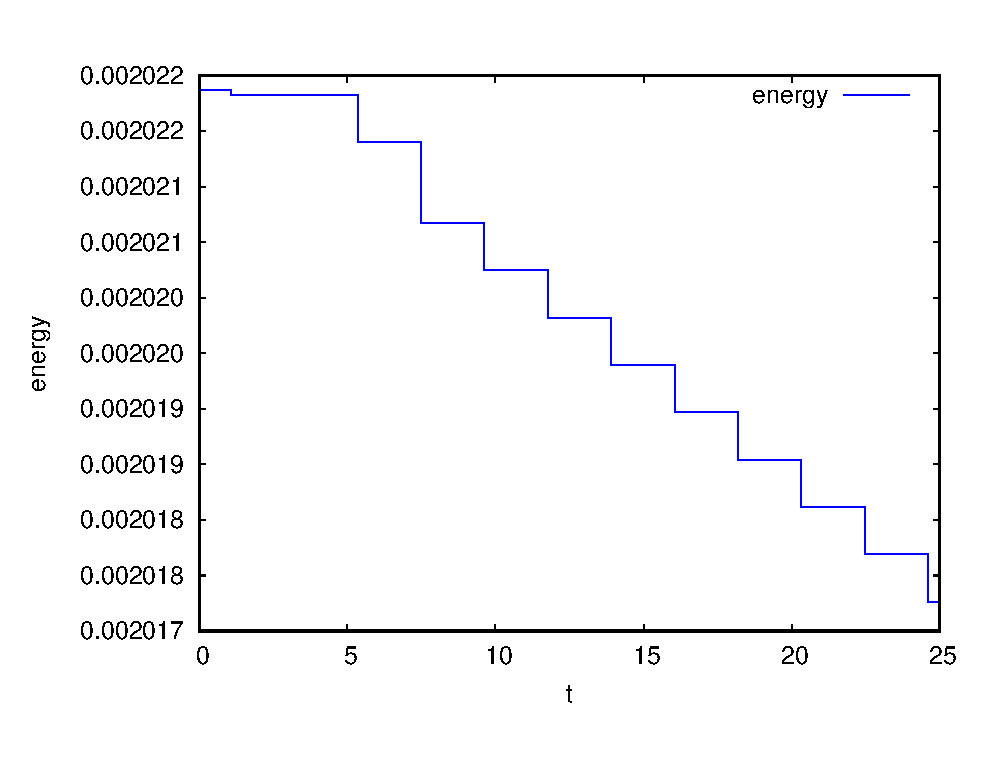
\includegraphics[scale=0.33]{content/pic/self_rot_25/kin_en.eps}
%        \caption{Кинетическая энергия}
%        \label{fig:self_rot_25_kin_en}
%    }
%    \hspace{10pt}
%    \subf{0.3\textwidth}{
%        \centering
%        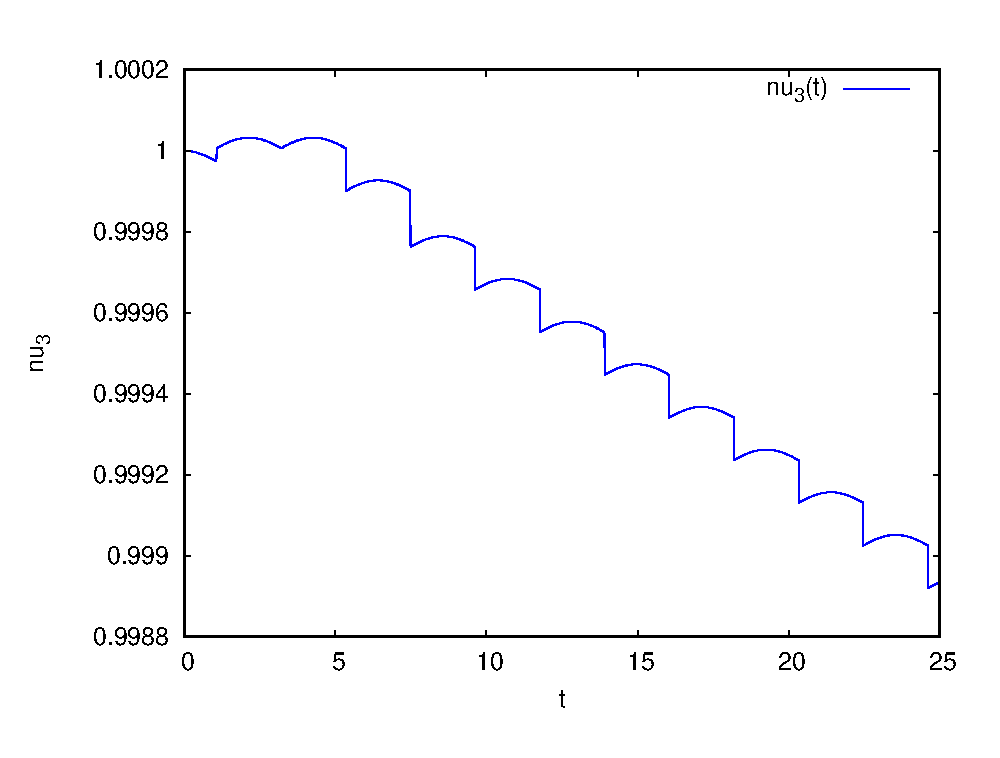
\includegraphics[scale=0.33]{content/pic/self_rot_25/nu3.eps}
%        \caption{Угловая скорость экипажа}
%        \label{fig:self_rot_25_nu3}
%    }
%    \hspace{10pt}
%    \subf{0.3\textwidth}{
%        \centering
%        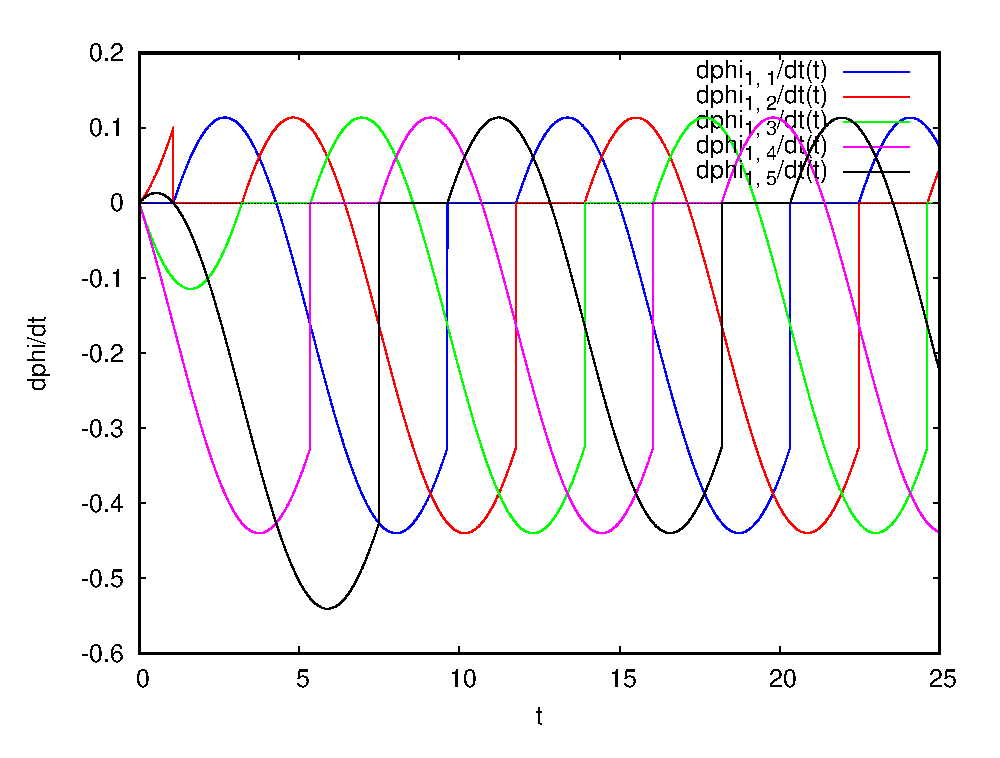
\includegraphics[scale=0.33]{content/pic/self_rot_25/rol_vel.eps}
%        \caption{Угловые скорости роликов}
%        \label{fig:self_rot_25_rol_vel}
%    }
%    \newline
%    \subf{0.3\textwidth}{
%        \centering
%        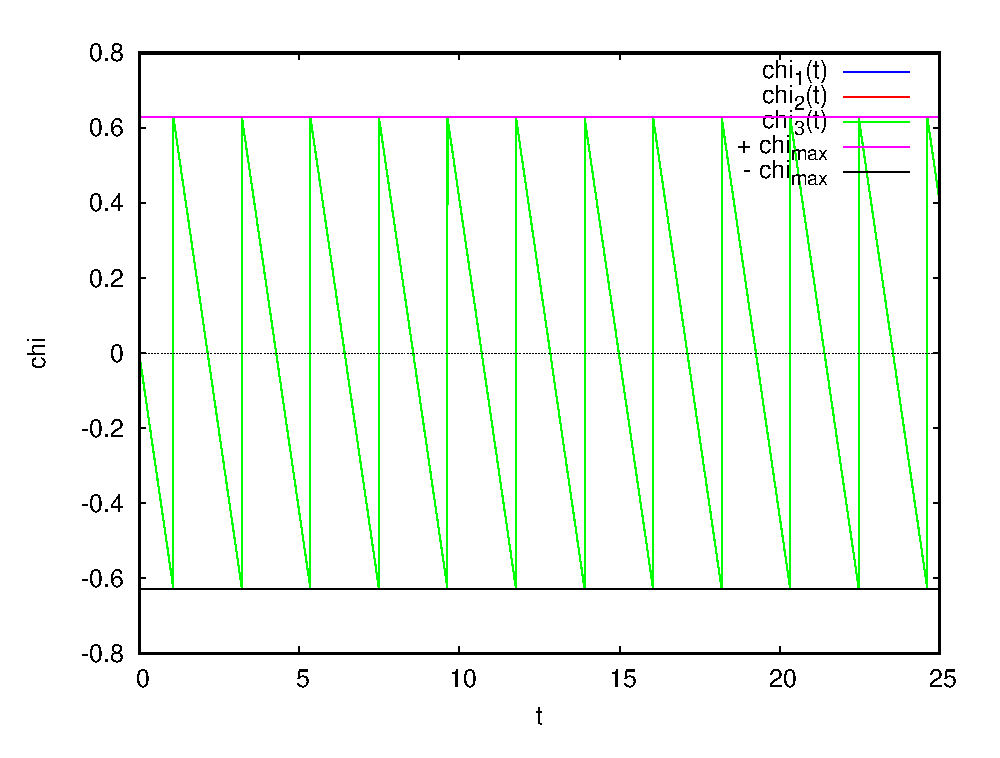
\includegraphics[scale=0.33]{content/pic/self_rot_25/chi.eps}
%        \caption{Углы поворота колес}
%        \label{fig:self_rot_25_chi}
%    }
%    \hspace{10pt}
%    \subf{0.3\textwidth}{
%        \centering
%        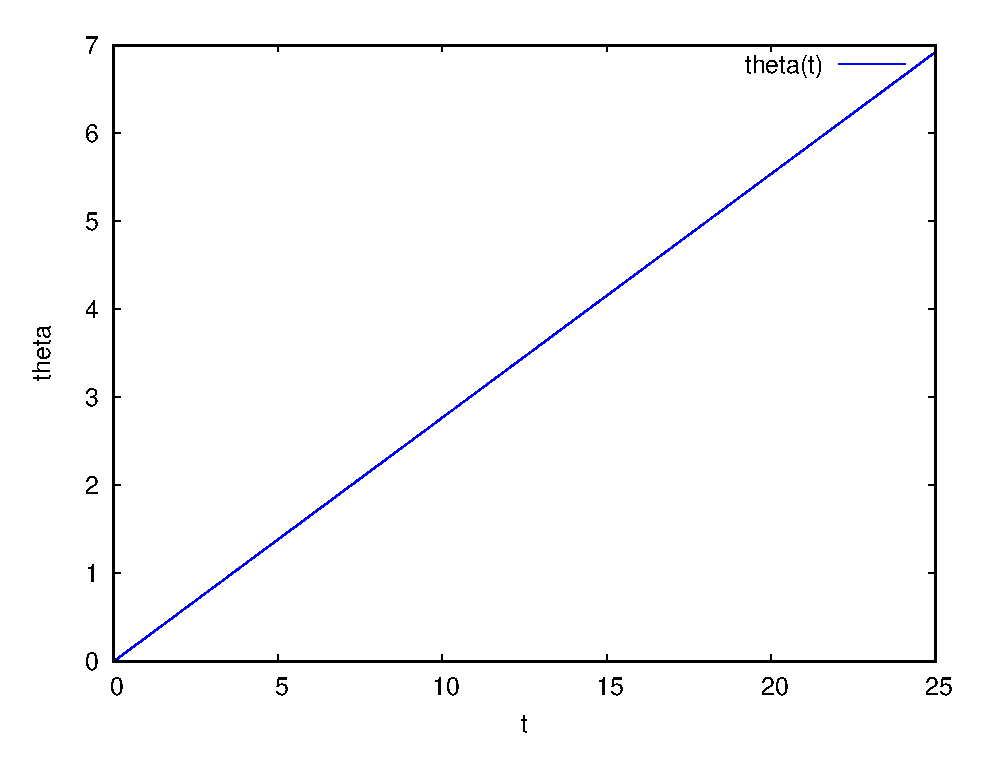
\includegraphics[scale=0.33]{content/pic/self_rot_25/theta.eps}
%        \caption{Угол поворота экипажа}
%        \label{fig:self_rot_25_theta}
%    }
%    \hspace{10pt}
%    \subf{0.3\textwidth}{
%        \centering
%        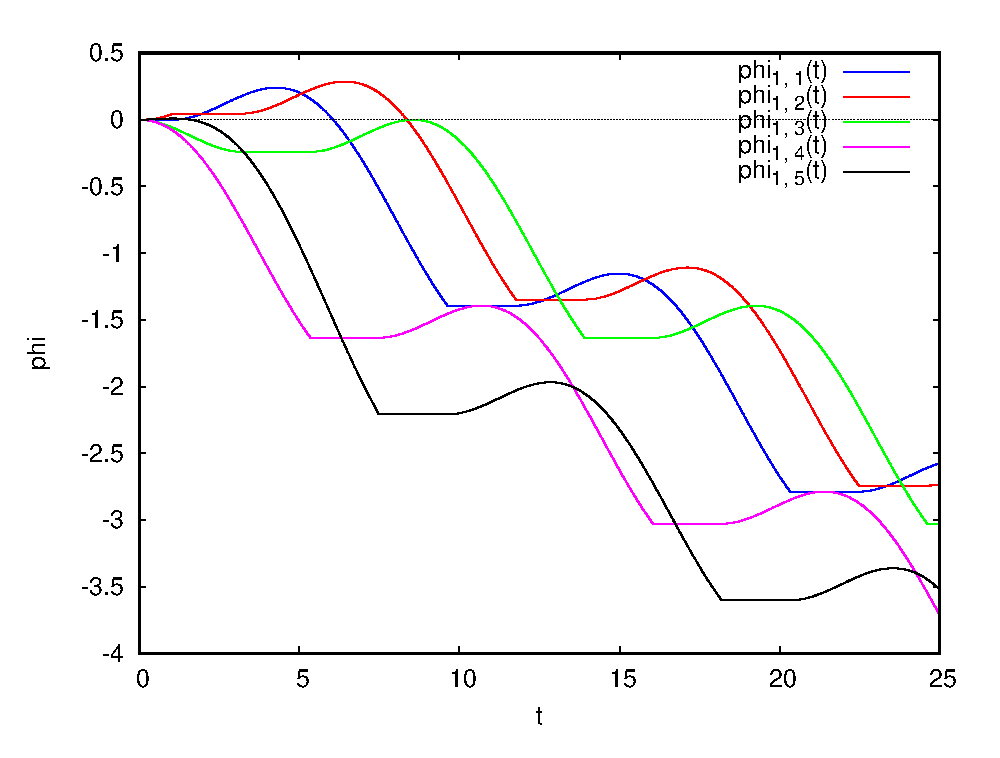
\includegraphics[scale=0.33]{content/pic/self_rot_25/rol_ang.eps}
%        \caption{Углы поворота роликов}
%        \label{fig:self_rot_25_rol_ang}
%    }
%    \caption{Вращение экипажа вокруг своей оси}
%\end{figure}
%\label{fig:self_rot}
%
%\newpage
%
% \subsection{По прямой}
%
%\begin{figure}[h]
%    \hspace{-20pt}
%    \subf{0.22\textwidth}{
%        \centering
%        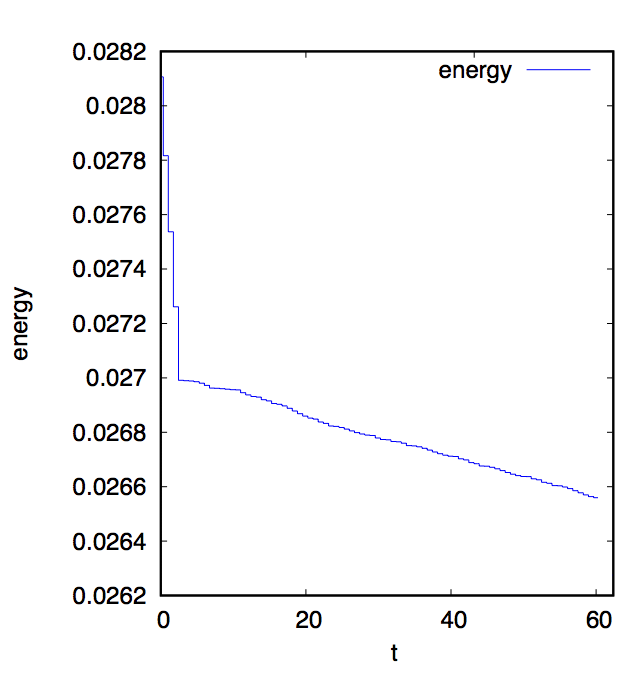
\includegraphics[scale=0.22]{content/pic/straight_60/kin_en.png}
%        \caption{Кинетическая энергия}
%        \label{fig:straight_60_kin_en}
%    }
%    \hspace{20pt}
%    \subf{0.4\textwidth}{
%        \centering
%        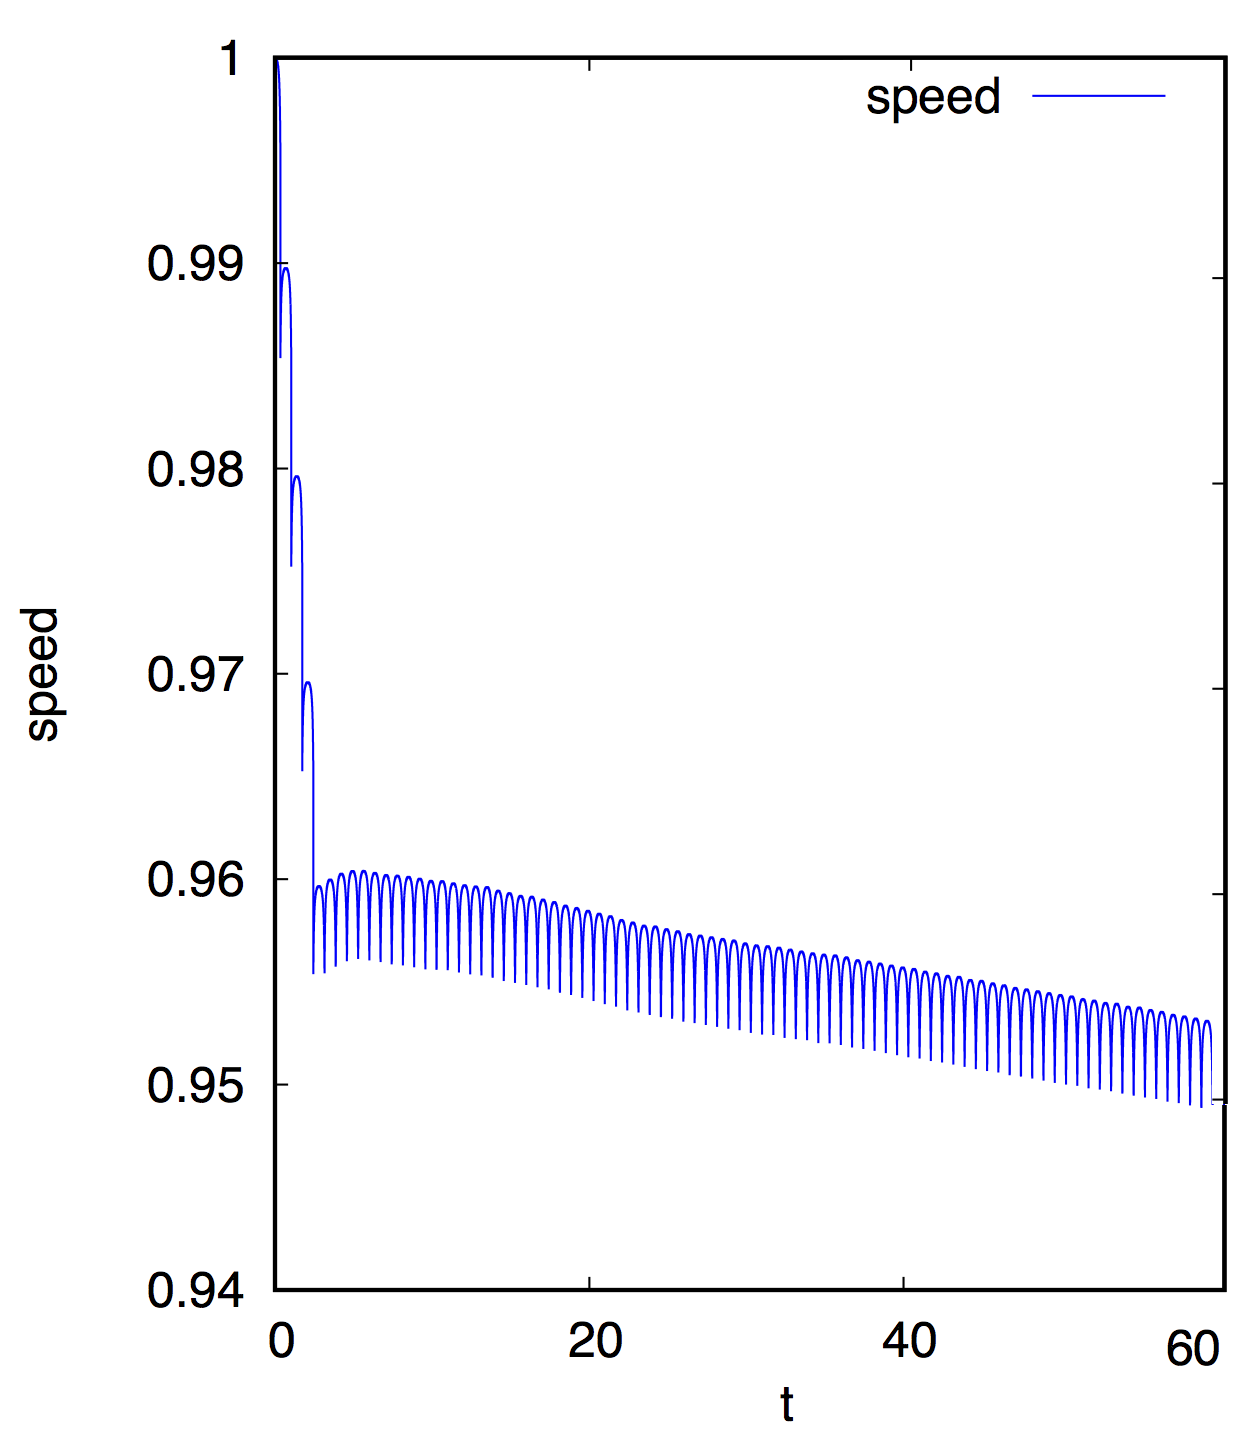
\includegraphics[scale=0.43]{content/pic/straight_60/v.png}
%        \caption{Скорость центра масс}
%        \label{fig:straight_60_v}
%    }
%    % \hspace{10pt}
%    \subf{0.35\textwidth}{
%        \centering
%        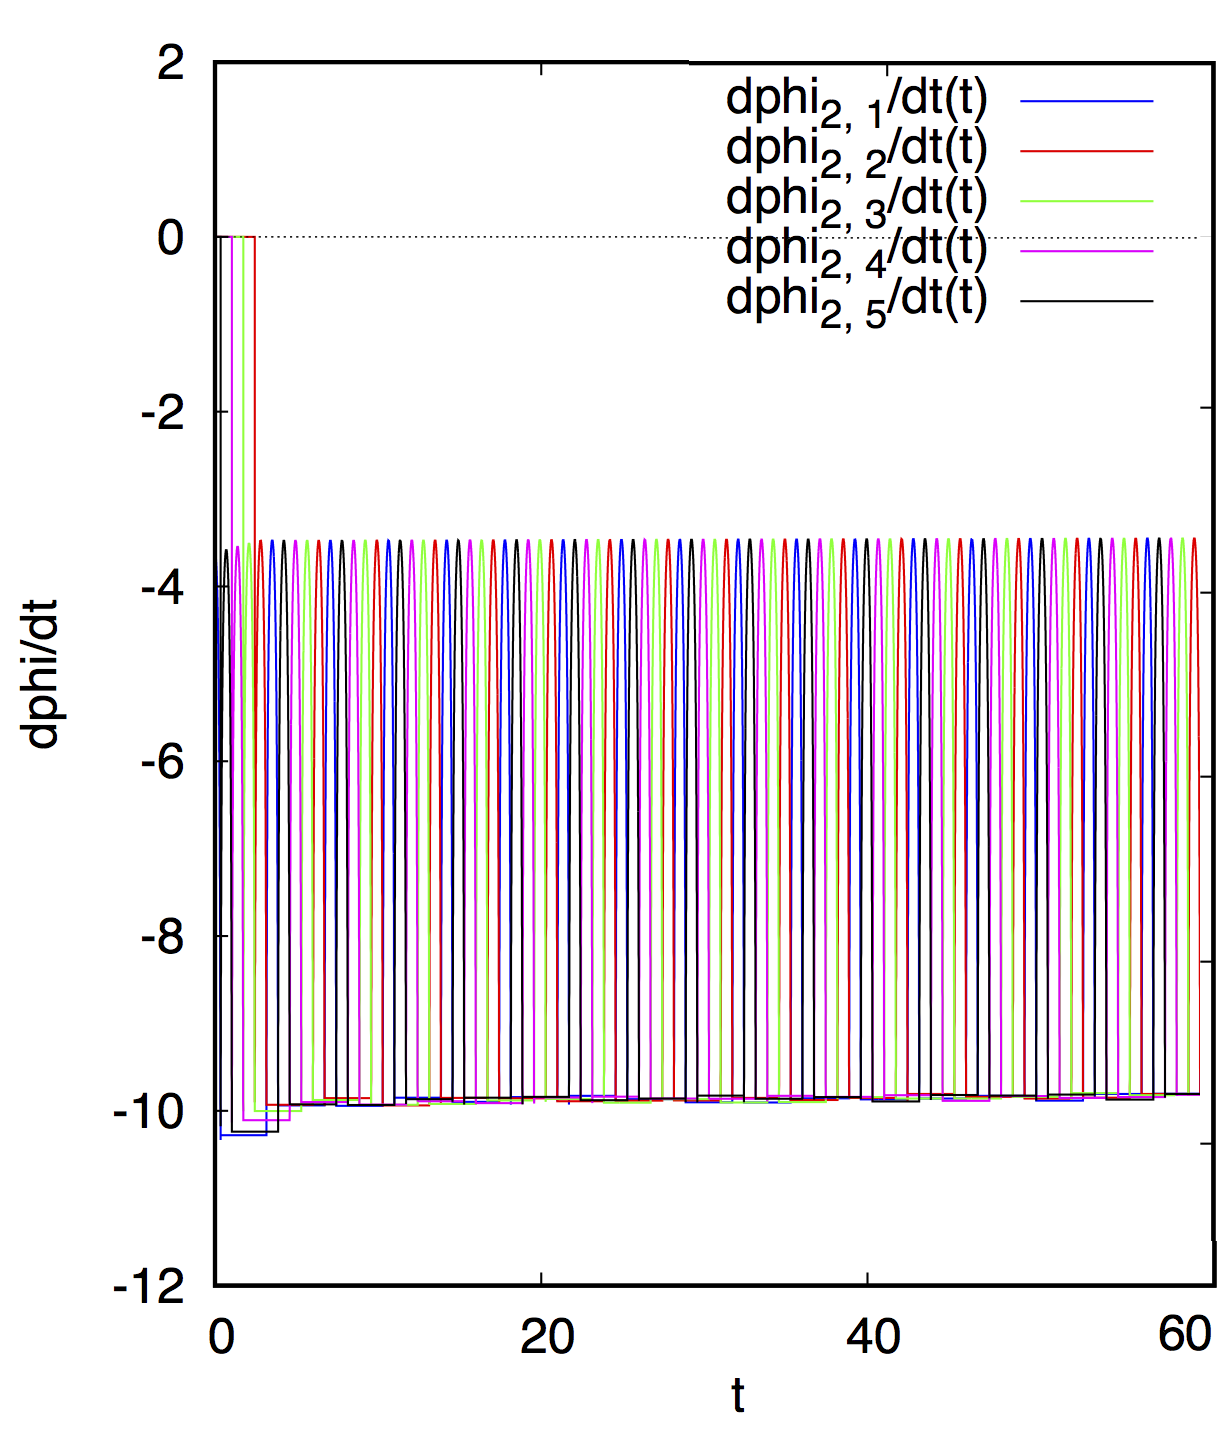
\includegraphics[scale=0.38]{content/pic/straight_60/nus2.png}
%        \caption{Угловые скорости роликов на заднем колесе}
%        \label{fig:straight_60_nus2}
%    }
%    \newline
%    \subf{0.3\textwidth}{
%        \centering
%        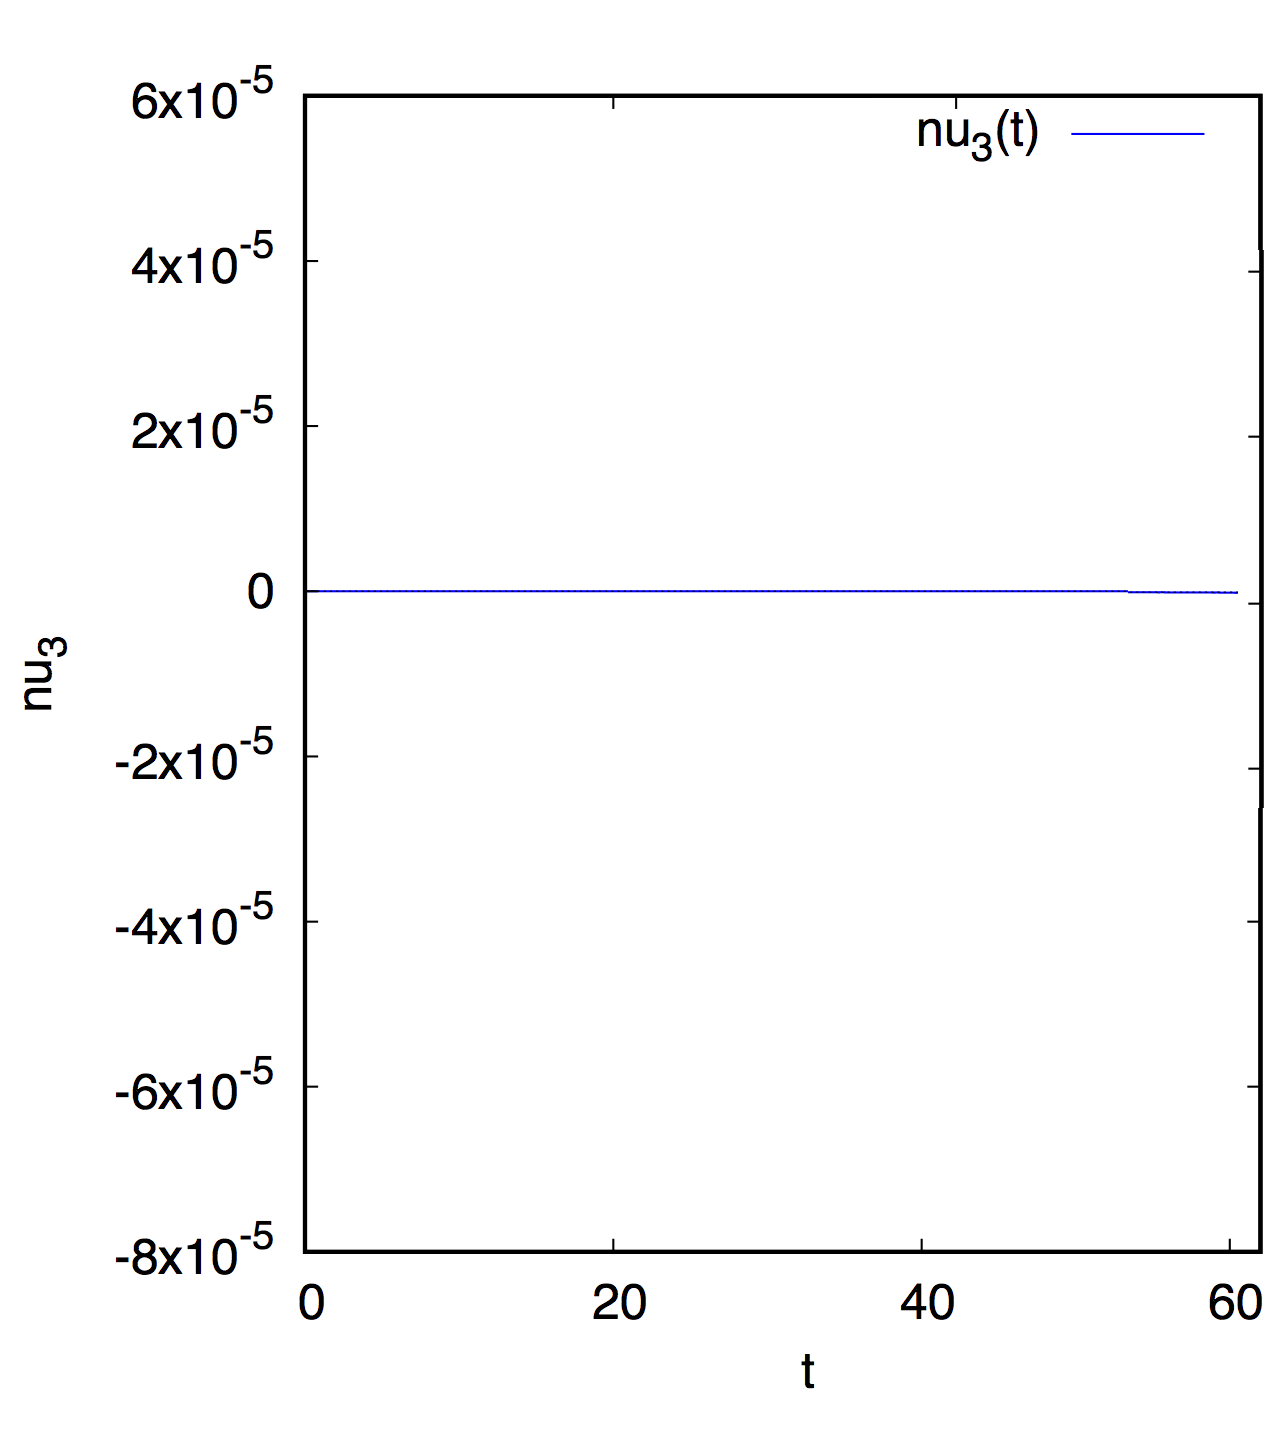
\includegraphics[scale=0.36]{content/pic/straight_60/nu3.png}
%        \caption{Угловая скорость экипажа}
%        \label{fig:straight_60_nu3}
%    }
%    \hspace{10pt}
%    \subf{0.3\textwidth}{
%        \centering
%        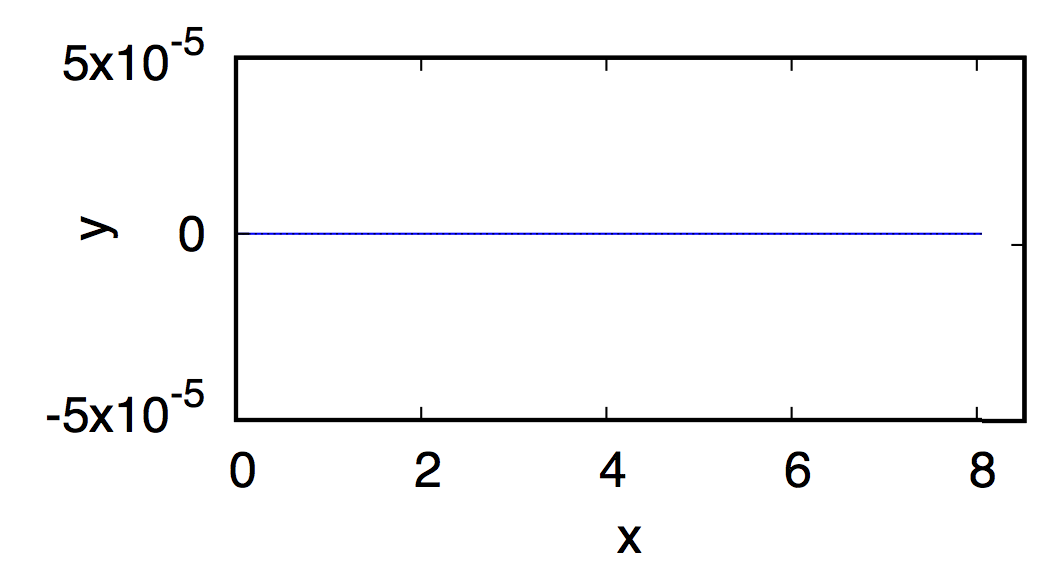
\includegraphics[scale=0.55]{content/pic/straight_60/traj.png}
%        \caption{Траектория}
%        \label{fig:straight_60_traj}
%    }
%    \hspace{10pt}
%    \subf{0.3\textwidth}{
%        \centering
%        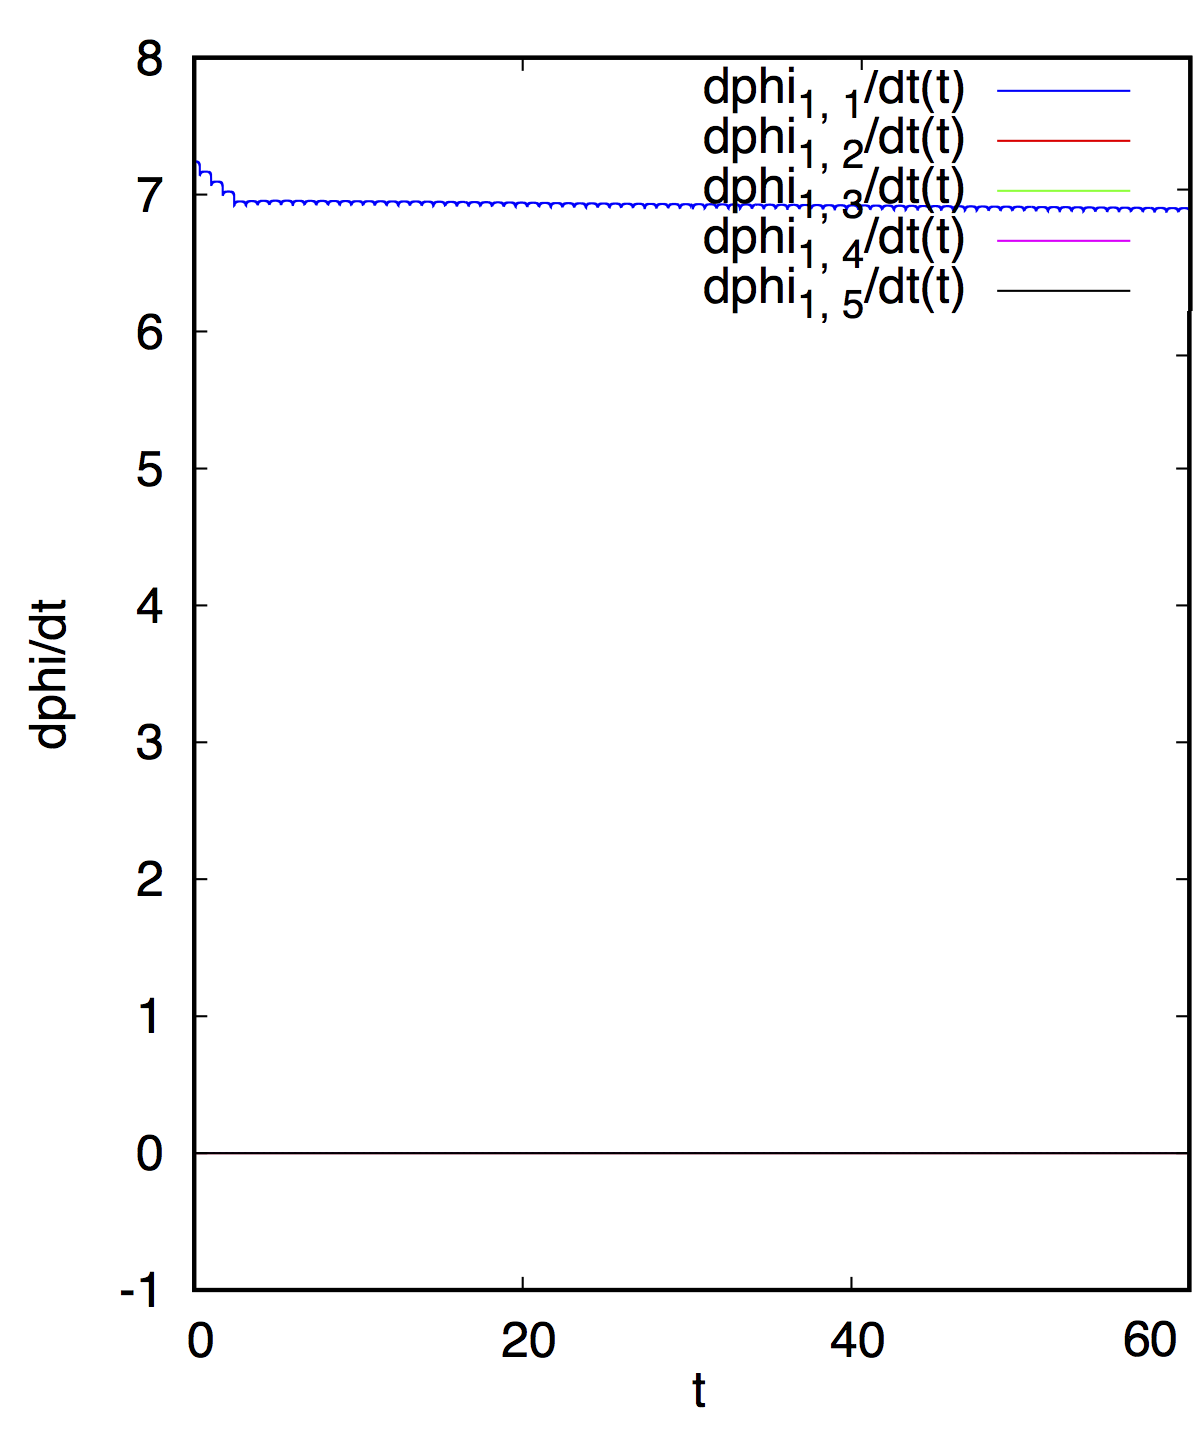
\includegraphics[scale=0.33]{content/pic/straight_60/nus1.png}
%        \caption{Угловые скорости роликов на переднем колесе}
%        \label{fig:straight_60_nus1}
%    }
%    \newline
%    \subf{0.3\textwidth}{
%        \centering
%        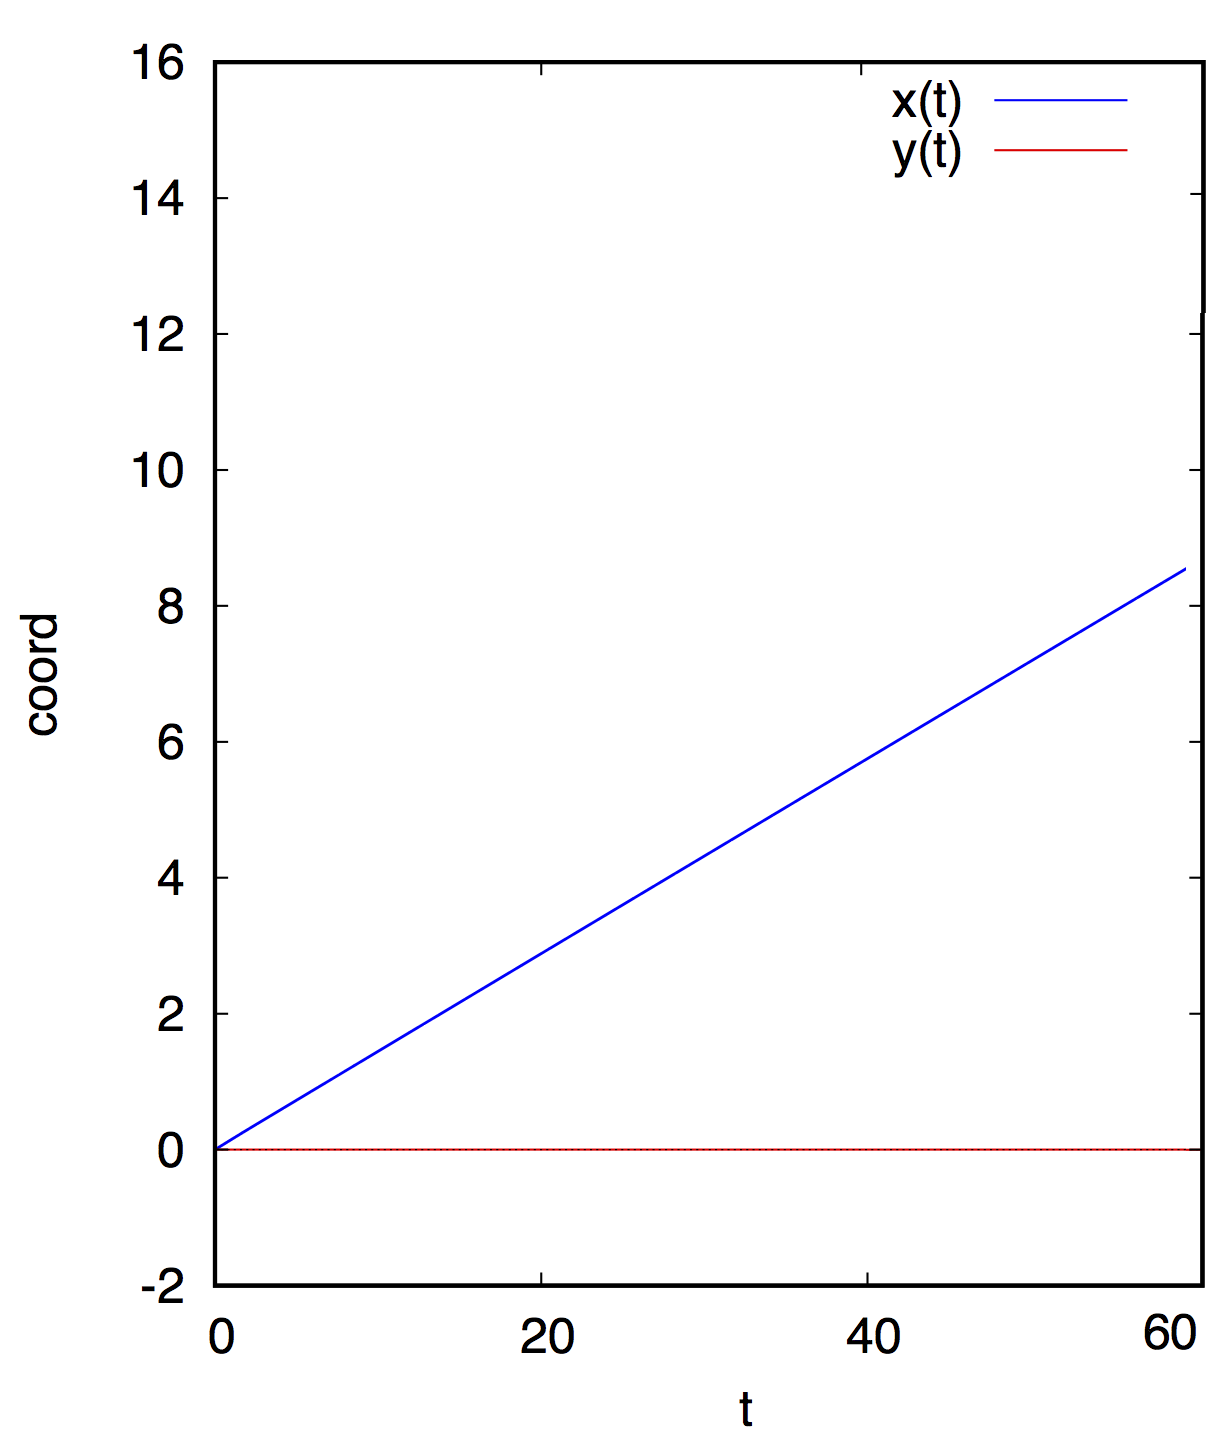
\includegraphics[scale=0.33]{content/pic/straight_60/xy.png}
%        \caption{Координаты центра масс}
%        \label{fig:straight_60_xy}
%    }
%    \hspace{10pt}
%    \subf{0.3\textwidth}{
%        \centering
%        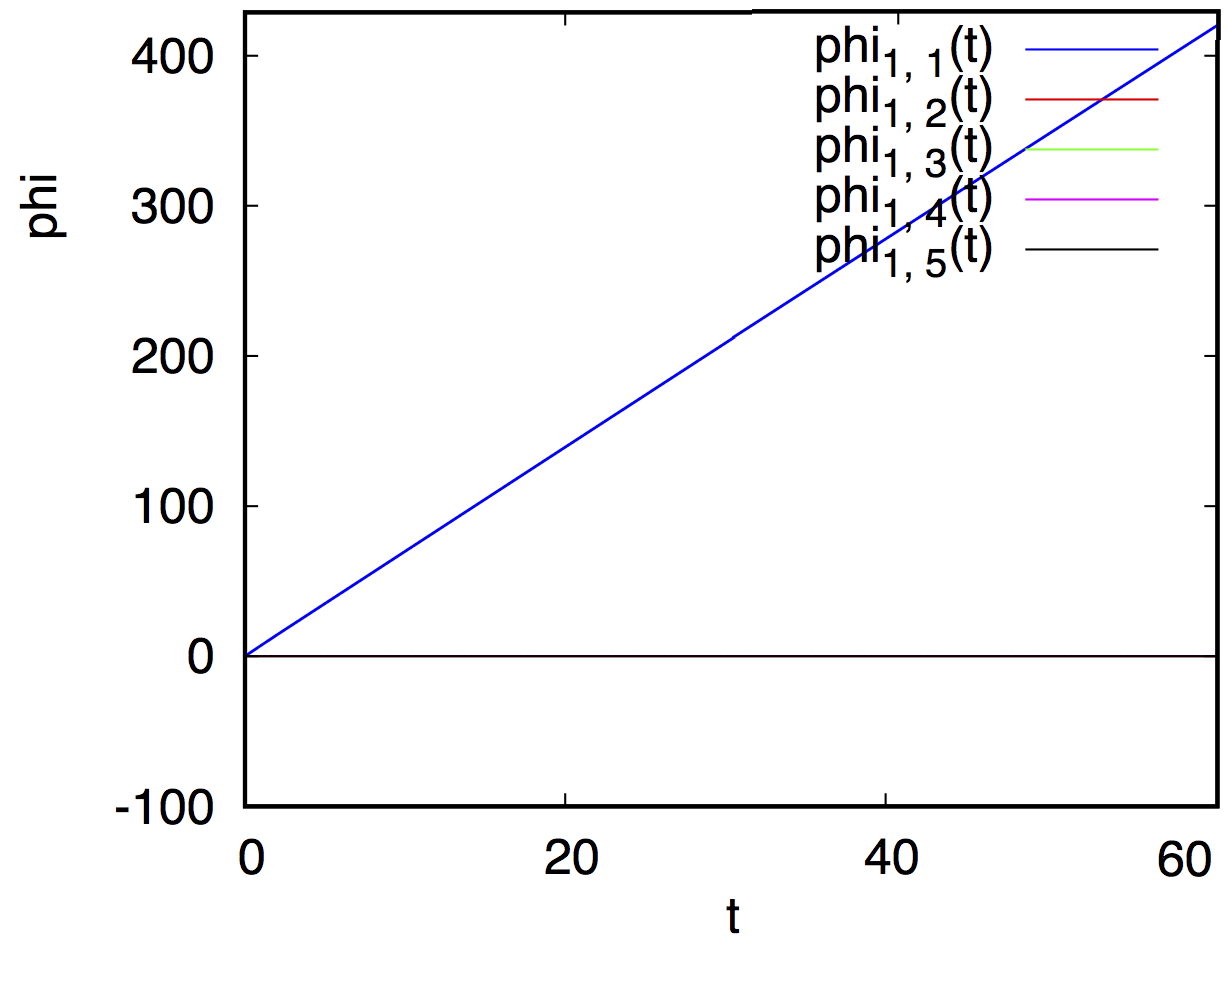
\includegraphics[scale=0.43]{content/pic/straight_60/phi1.png}
%        \caption{Углы поворота роликов на переднем колесе}
%        \label{fig:straight_60_phi1}
%    }
%    \hspace{10pt}
%    \subf{0.3\textwidth}{
%        \centering
%        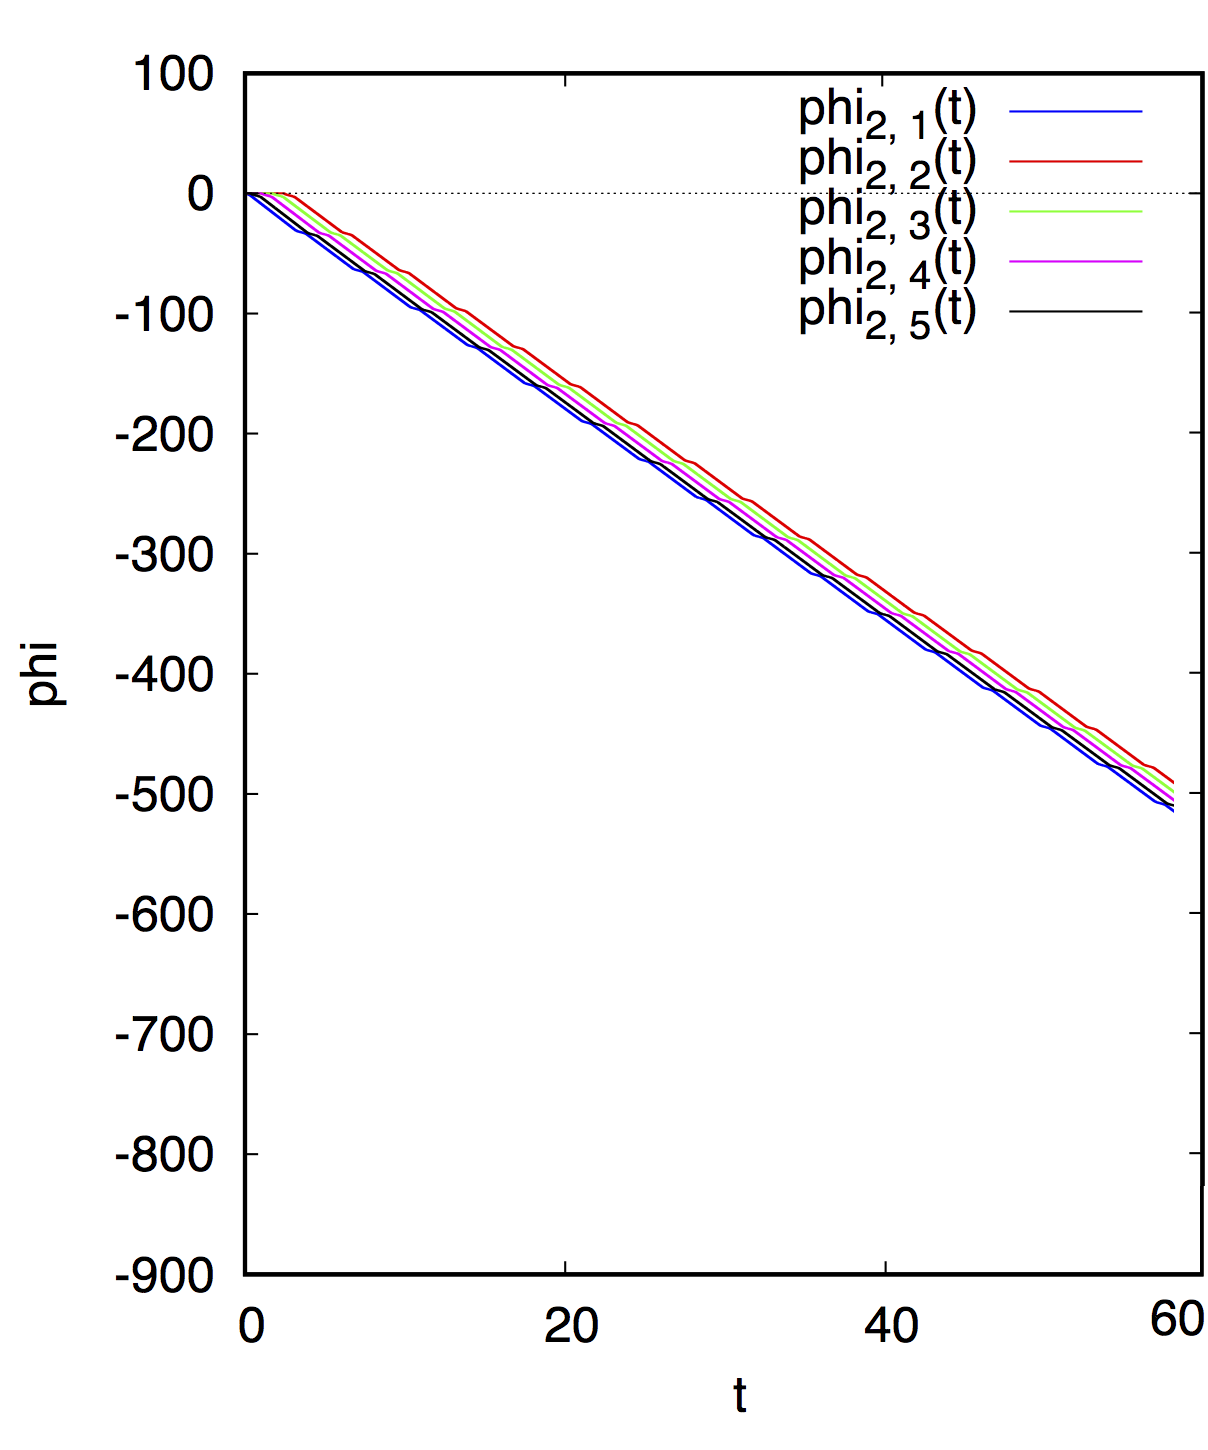
\includegraphics[scale=0.33]{content/pic/straight_60/phi2.png}
%        \caption{Углы поворота роликов на заднем колесе}
%        \label{fig:straight_60_phi2}
%    }
%    \caption{Движение экипажа по прямой}
%\end{figure}
%\label{fig:straight}
%
%\newpage
%
% \subsection{С закруткой}
%
%\begin{figure}[h]
%    \subf{0.3\textwidth}{
%        \centering
%        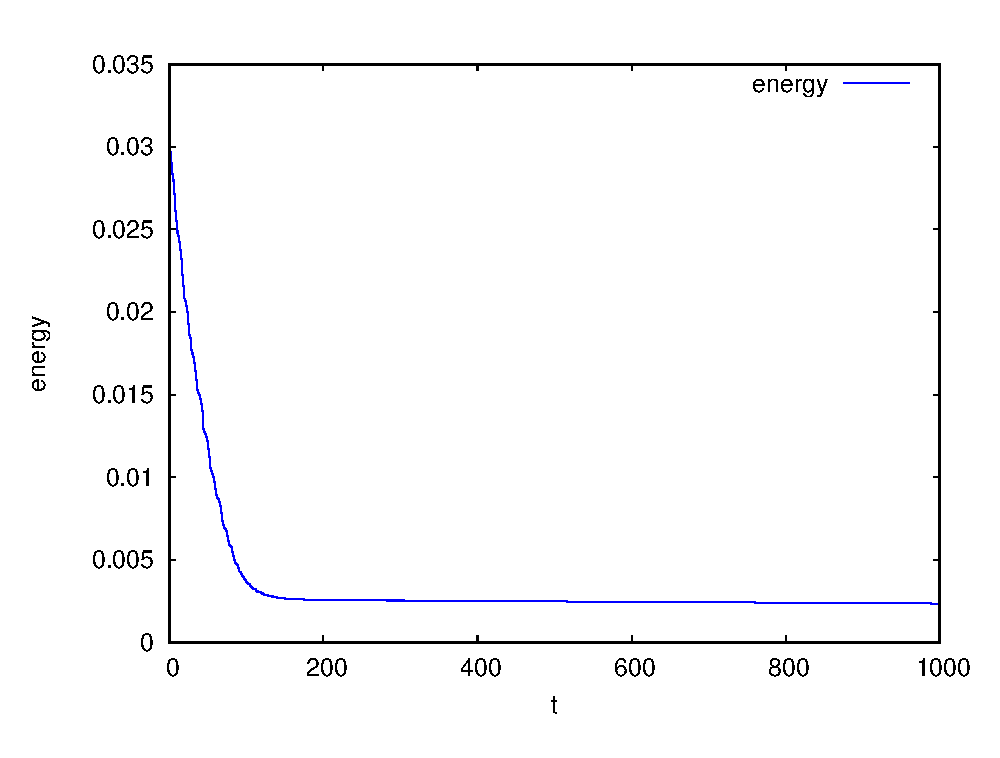
\includegraphics[scale=0.33]{content/pic/wrench_1000/kin_en.eps}
%        \caption{Кинетическая энергия}
%        \label{fig:wrench_1000_kin_en}
%    }
%    \hspace{10pt}
%    \subf{0.3\textwidth}{
%        \centering
%        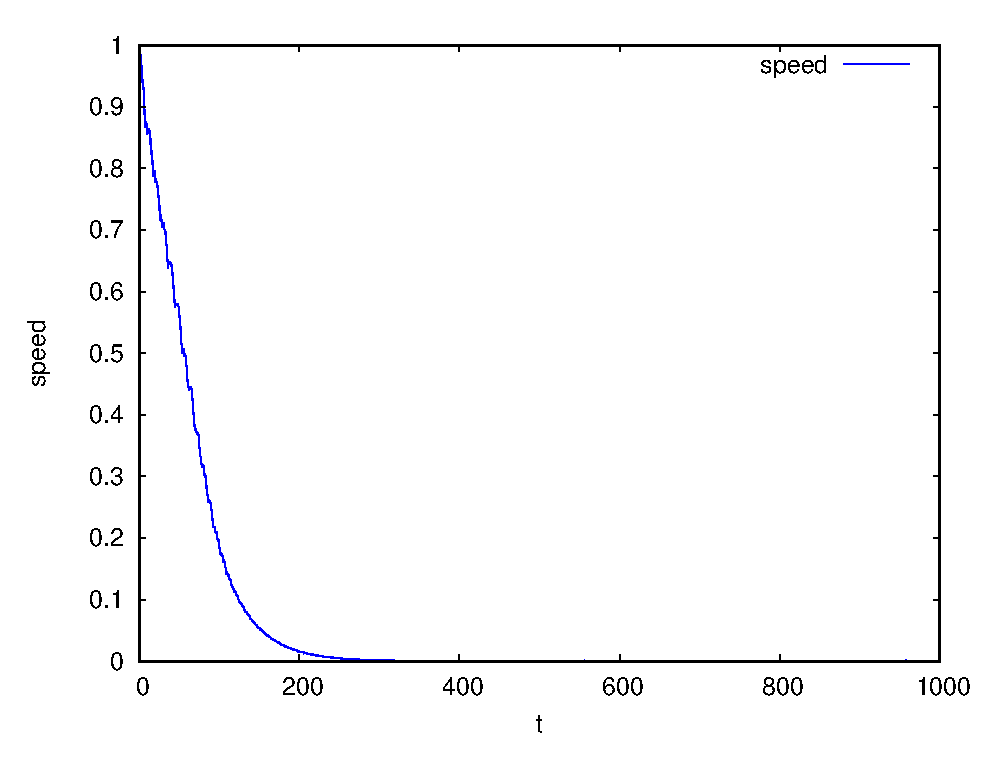
\includegraphics[scale=0.33]{content/pic/wrench_1000/v.eps}
%        \caption{Скорость центра масс}
%        \label{fig:wrench_1000_v}
%    }
%    \hspace{10pt}
%    \subf{0.3\textwidth}{
%        \centering
%        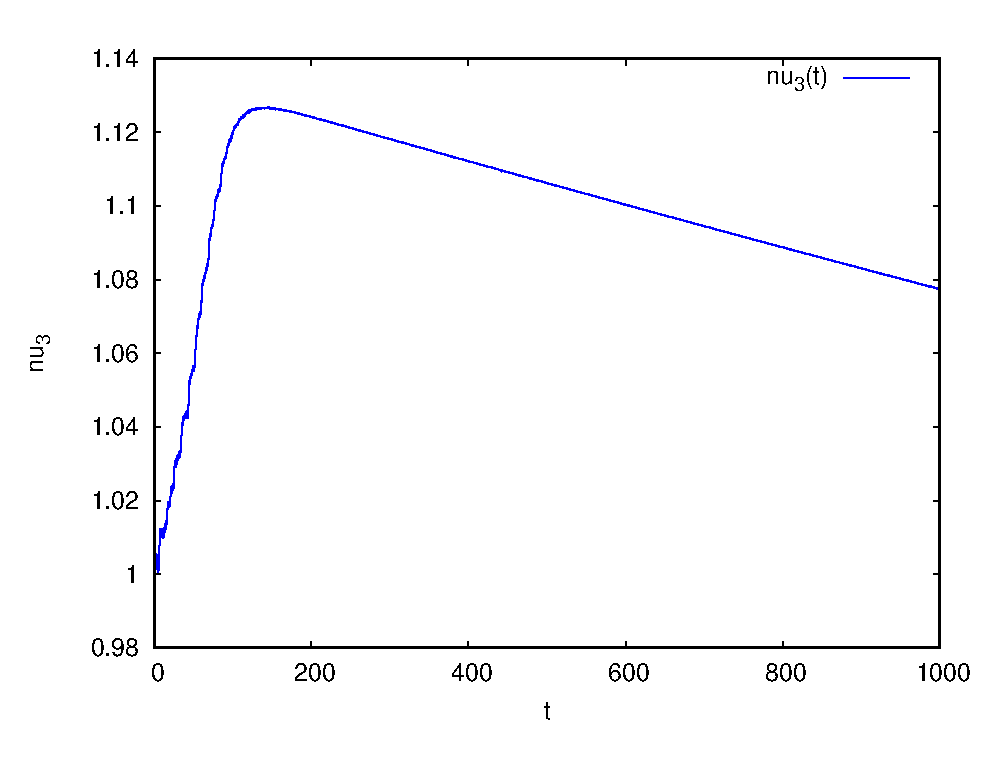
\includegraphics[scale=0.33]{content/pic/wrench_1000/nu3.eps}
%        \caption{Угловая скорость экипажа}
%        \label{fig:wrench_1000_nu3}
%    }
%    \newline
%    \subf{0.45\textwidth}{
%        \centering
%        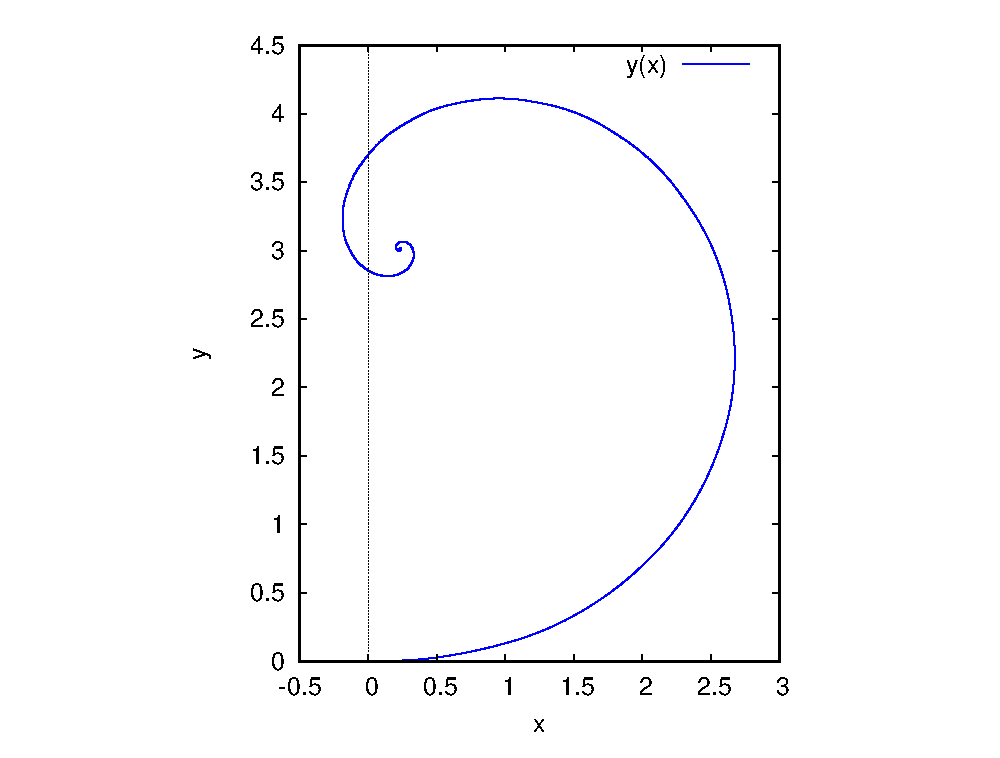
\includegraphics[scale=0.33]{content/pic/wrench_1000/traj.eps}
%        \caption{Траектория центра масс}
%        \label{fig:wrench_1000_traj}
%    }
%    \hspace{10pt}
%    \subf{0.45\textwidth}{
%        \centering
%        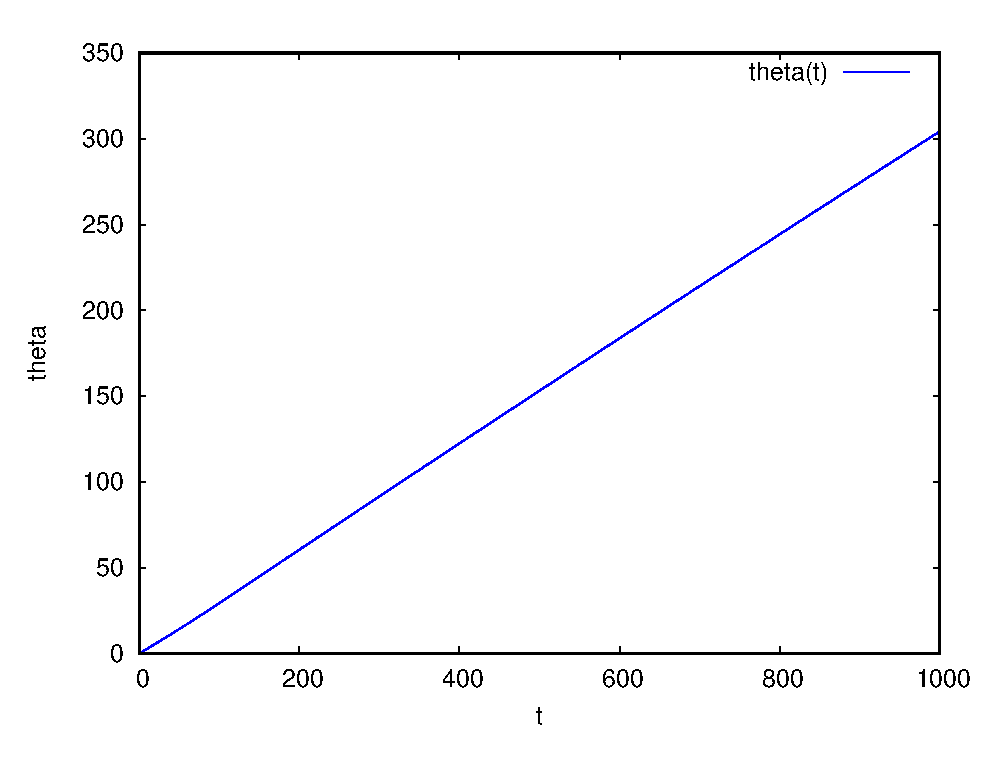
\includegraphics[scale=0.33]{content/pic/wrench_1000/theta.eps}
%        \caption{Угол поворота экипажа}
%        \label{fig:wrench_1000_theta}
%    }
%    \newline
%    \subf{0.45\textwidth}{
%        \centering
%        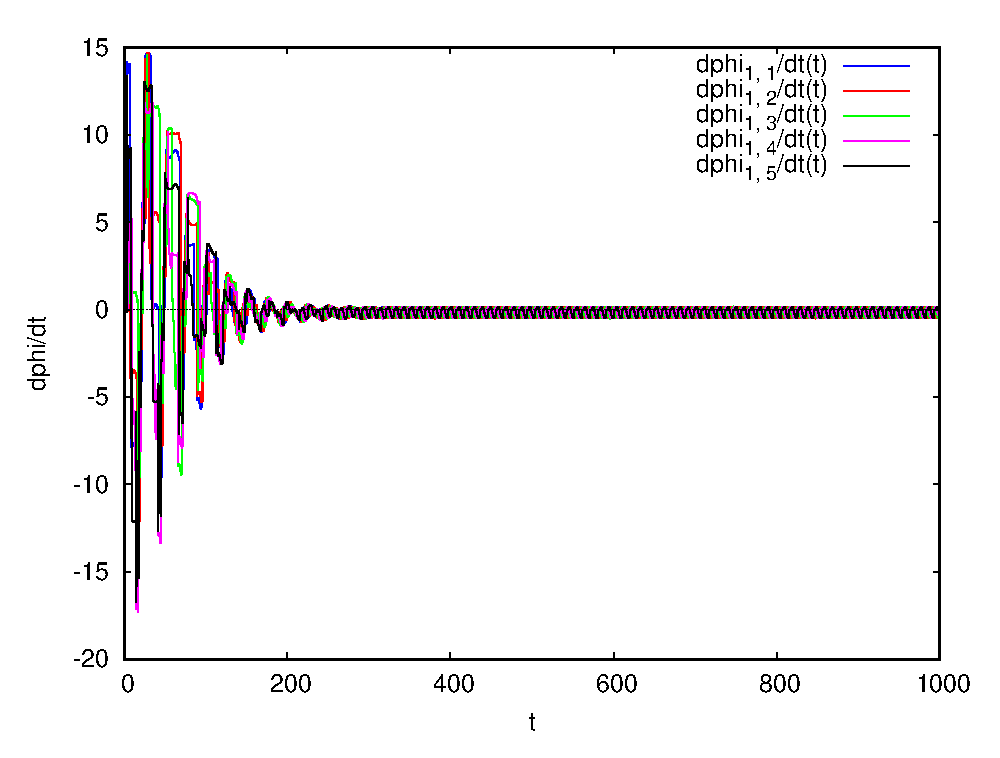
\includegraphics[scale=0.33]{content/pic/wrench_1000/nus1.eps}
%        \caption{Угловые скорости роликов на переднем колесе}
%        \label{fig:wrench_1000_nus1}
%    }
%    \hspace{10pt}
%    \subf{0.45\textwidth}{
%        \centering
%        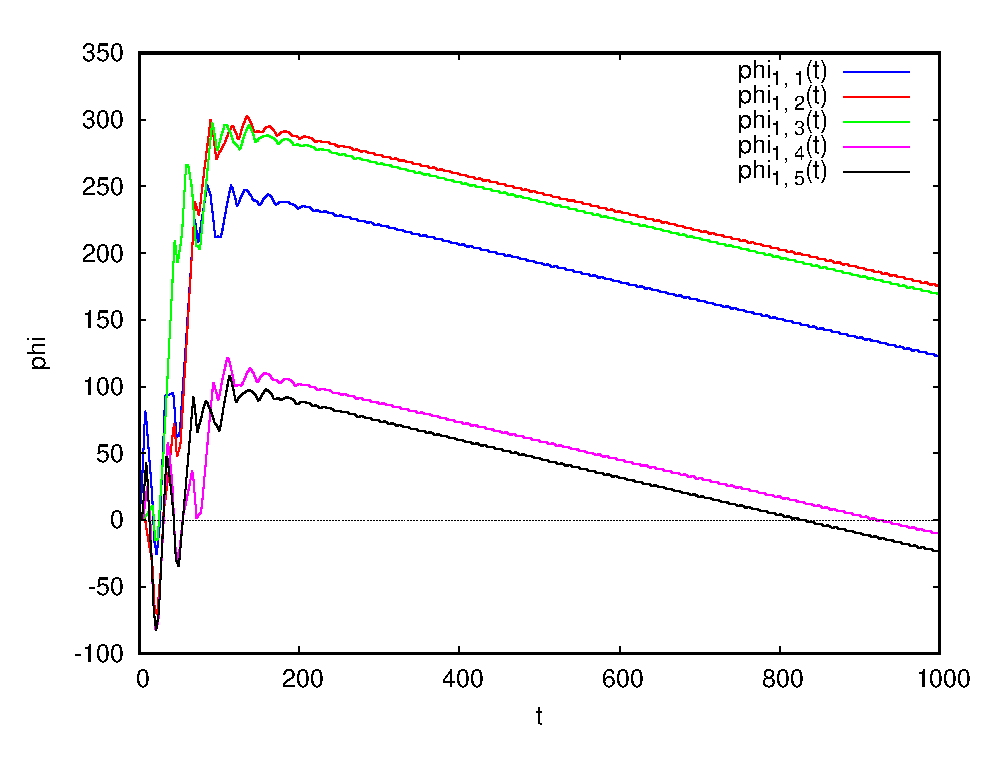
\includegraphics[scale=0.33]{content/pic/wrench_1000/phi1.eps}
%        \caption{Углы поворота роликов на переднем колесе}
%        \label{fig:wrench_1000_phi1}
%    }
%    \caption{Движение экипажа с закруткой}
%\end{figure}
%\label{fig:wrench}
%
